\documentclass{article}[10pt]
\usepackage{multicol, enumerate, enumitem, hyperref, color, soul, setspace, parskip, fancyhdr, amssymb, amsthm, amsmath, bbm, latexsym, units, mathtools}
\everymath{\displaystyle}
\usepackage[headsep=0.5cm,headheight=0cm, left=1 in,right= 1 in,top= 1 in,bottom= 1 in]{geometry}

\begin{document}
This is the Answer Key for Module 7 Version B.

31. Determine the domain of the function below.
$$ \frac{4}{20 x^2 - 41 x + 20} $$ 
The solution is $ \text{All Real numbers except } x = a \text{ and } x = b, \text{ where } a \in [0.33, 0.91] \text{ and } b \in [0.97, 1.6] $ 

\begin{enumerate}[label=\Alph*.] 
\item $ \text{All Real numbers except } x = a \text{ and } x = b, \text{ where } a \in [0.33, 0.91] \text{ and } b \in [0.97, 1.6] $ 

 This is the correct option! 
\item $ \text{All Real numbers except } x = a \text{ and } x = b, \text{ where } a \in [19.73, 20.01] \text{ and } b \in [19.73, 20.01] $ 

 This corresponds to not factoring the denominator correctly. 
\item $ \text{All Real numbers except } x = a, \text{ where } a \in [0.33, 0.91] $ 

 This corresponds to removing only 1 value from the denominator. 
\item $ \text{All Real numbers except } x = a, \text{ where } a \in [19.73, 20.01] $ 

 This corresponds to removing a distractor value from the denominator. 
\item $ \text{All Real numbers.} $ 

 This corresponds to thinking the denominator has complex roots or that rational functions have a domain of all Real numbers. 
\end{enumerate} 
 
General Comments: The new domain is the intersection of the previous domains.

-----------------------------------------------

32. Solve the rational equation below. Then, choose the interval(s) that the solution(s) belongs to.
$$ \frac{-5}{4*x + 4} - -3 = \frac{7}{-16*x - 16} $$ 
The solution is $ -0.729166666667 $ 

\begin{enumerate}[label=\Alph*.] 
\item $ x \in [0.84,1.29] $ 

  
\item $ x_1 \in [-0.27, 0.24] \text{ and } x_2 \in [-2,0] $ 

  
\item $ \text{All solutions lead to invalid or complex values in the equation.} $ 

  
\item $ x_1 \in [0.84, 1.29] \text{ and } x_2 \in [-2,0] $ 

  
\item $ x \in [-0.89,-0.43] $ 

  
\end{enumerate} 
 
General Comments: Distractors are different based on the number of solutions. Remember that after solving, we need to make sure our solution does not make the original equation divide by zero!

-----------------------------------------------

33. Solve the rational equation below. Then, choose the interval(s) that the solution(s) belongs to.
$$ -3*x/(7*x + 3) - 6*x**2/(-42*x**2 + 31*x + 21) = 5/(-6*x + 7) $$ 
The solution is $ [7/3 + sqrt(241)/6, -sqrt(241)/6 + 7/3] $ 

\begin{enumerate}[label=\Alph*.] 
\item $ x_1 \in [4.6, 6.4] \text{ and } x_2 \in [-0.87,0.16] $ 

  
\item $ x \in [-4.5,0.6] $ 

  
\item $ \text{All solutions lead to invalid or complex values in the equation.} $ 

  
\item $ x_1 \in [4.6, 6.4] \text{ and } x_2 \in [-1.54,-0.69] $ 

  
\item $ x \in [0.6,3.9] $ 

  
\end{enumerate} 
 
General Comments: Distractors are different based on the number of solutions. Remember that after solving, we need to make sure our solution does not make the original equation divide by zero!

-----------------------------------------------

34. Choose the equation of the function graphed below.
$$ \text{Graph of the function } f(x) = \frac{-1}{x + 2} - 3 $$ 
\begin{center}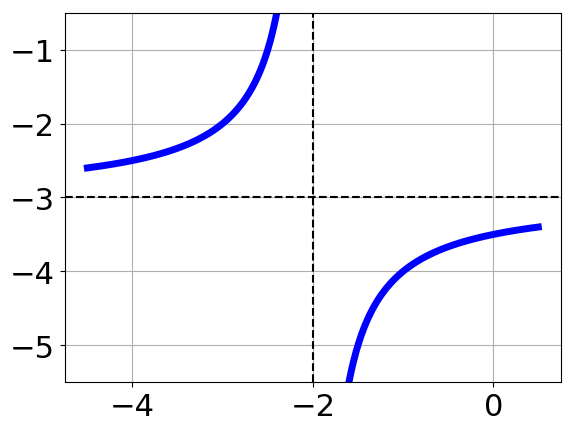
\includegraphics[scale=0.5]{../Figures/question34B.png}\end{center}The solution is $ \frac{-1}{x + 2} - 3 $ 

\begin{enumerate}[label=\Alph*.] 
\item $ \frac{1}{(x - 2)^2} - 3 $ 

 Corresponds to thinking the graph was a shifted version of $\frac{1}{x^2}$, using the general form $f(x) = \frac{a}{x+h}+k$, and the opposite leading coefficient. 
\item $ \frac{-1}{x + 2} - 3 $ 

 This is the correct option. 
\item $ \frac{1}{x - 2} - 3 $ 

 Corresponds to using the general form $f(x) = \frac{a}{x+h}+k$ and the opposite leading coefficient. 
\item $ \frac{-1}{(x + 2)^2} - 3 $ 

 Corresponds to thinking the graph was a shifted version of $\frac{1}{x^2}$. 
\end{enumerate} 
 
General Comments: Remember that the general form of a basic rational equation is $ f(x) = \frac{a}{(x-h)^n} + k$, where $a$ is the leading coefficient (and in this case, we assume is either $1$ or $-1$), $n$ is the degree (in this case, either $1$ or $2$), and $(h, k)$ is the intersection of the asymptotes.

-----------------------------------------------

35. Choose the graph of the equation below.
$$ \frac{-1}{x + 2} - 3 $$ 
The solution is  
\begin{center}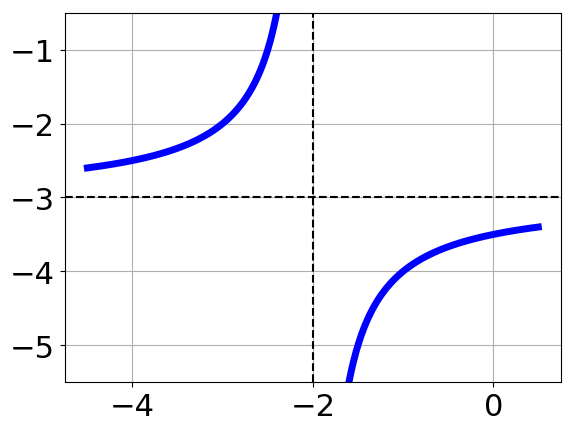
\includegraphics[scale=0.5]{../Figures/question35BB.png}\end{center}\begin{enumerate}[label=\Alph*.] 
\item  
\begin{center}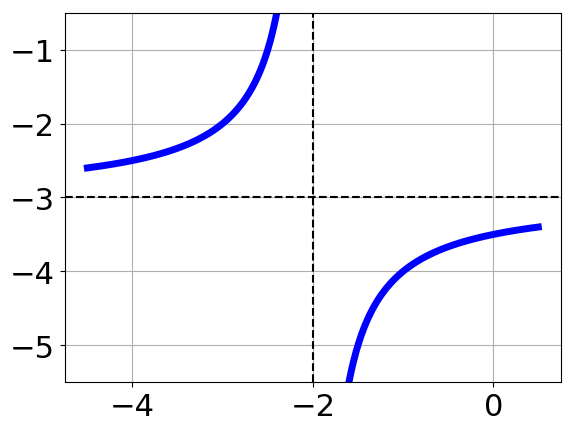
\includegraphics[scale=0.5]{../Figures/question35BB.png}\end{center} 
 
\item  
\begin{center}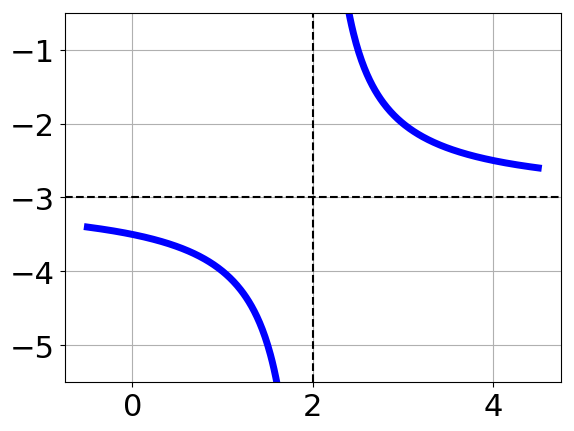
\includegraphics[scale=0.5]{../Figures/question35BD.png}\end{center} 
 
\item  
\begin{center}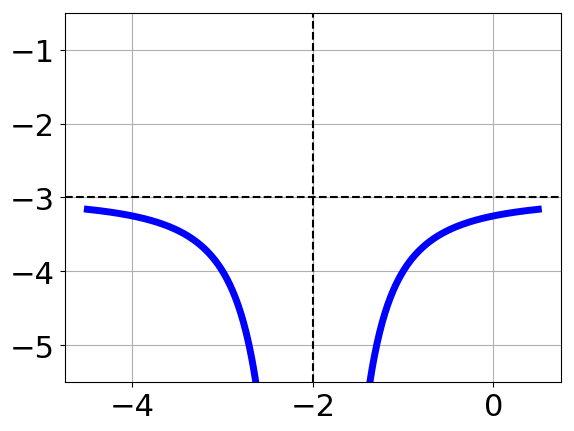
\includegraphics[scale=0.5]{../Figures/question35BA.png}\end{center} 
 
\item  
\begin{center}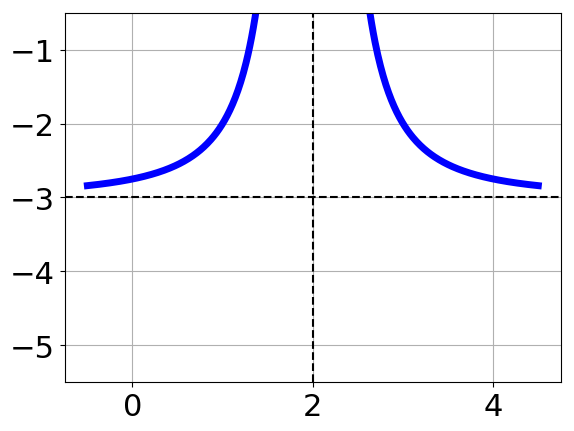
\includegraphics[scale=0.5]{../Figures/question35BC.png}\end{center} 
 
\end{enumerate} 
 
General Comments: Remember that the general form of a basic rational equation is $ f(x) = \frac{a}{(x-h)^n} + k$, where $a$ is the leading coefficient (and in this case, we assume is either $1$ or $-1$), $n$ is the degree (in this case, either $1$ or $2$), and $(h, k)$ is the intersection of the asymptotes.

-----------------------------------------------


\end{document}
